\documentclass{beamer}
\usepackage[T1]{fontenc}
\usepackage{minted}
\usepackage{graphicx}

%\setbeameroption{show notes on second screen}
\graphicspath{ {./images/} }
\usecolortheme{owl}
\usemintedstyle{monokai}
\definecolor{codebg}{rgb}{0.15,0.15,0.15}
\setminted{bgcolor=codebg,breaklines}

%Information to be included in the title page:
\title{CompSci Crash Course}
\author{Apples}
\institute{Comfy Gamedev}
\date{January 2023}

\newenvironment{xframe}[2][]
{
    \begin{frame}[fragile,environment=xframe,#1]
    \frametitle{#2}
}{
    \end{frame}
}

\AtBeginSection[]
{
\begin{frame}
    \frametitle{Table of Contents}
    \tableofcontents[currentsection]
    \note{(table of contents)}
\end{frame}
}

\begin{document}

\frame{\titlepage}

\begin{xframe}{When I Say "Crash Course"}
    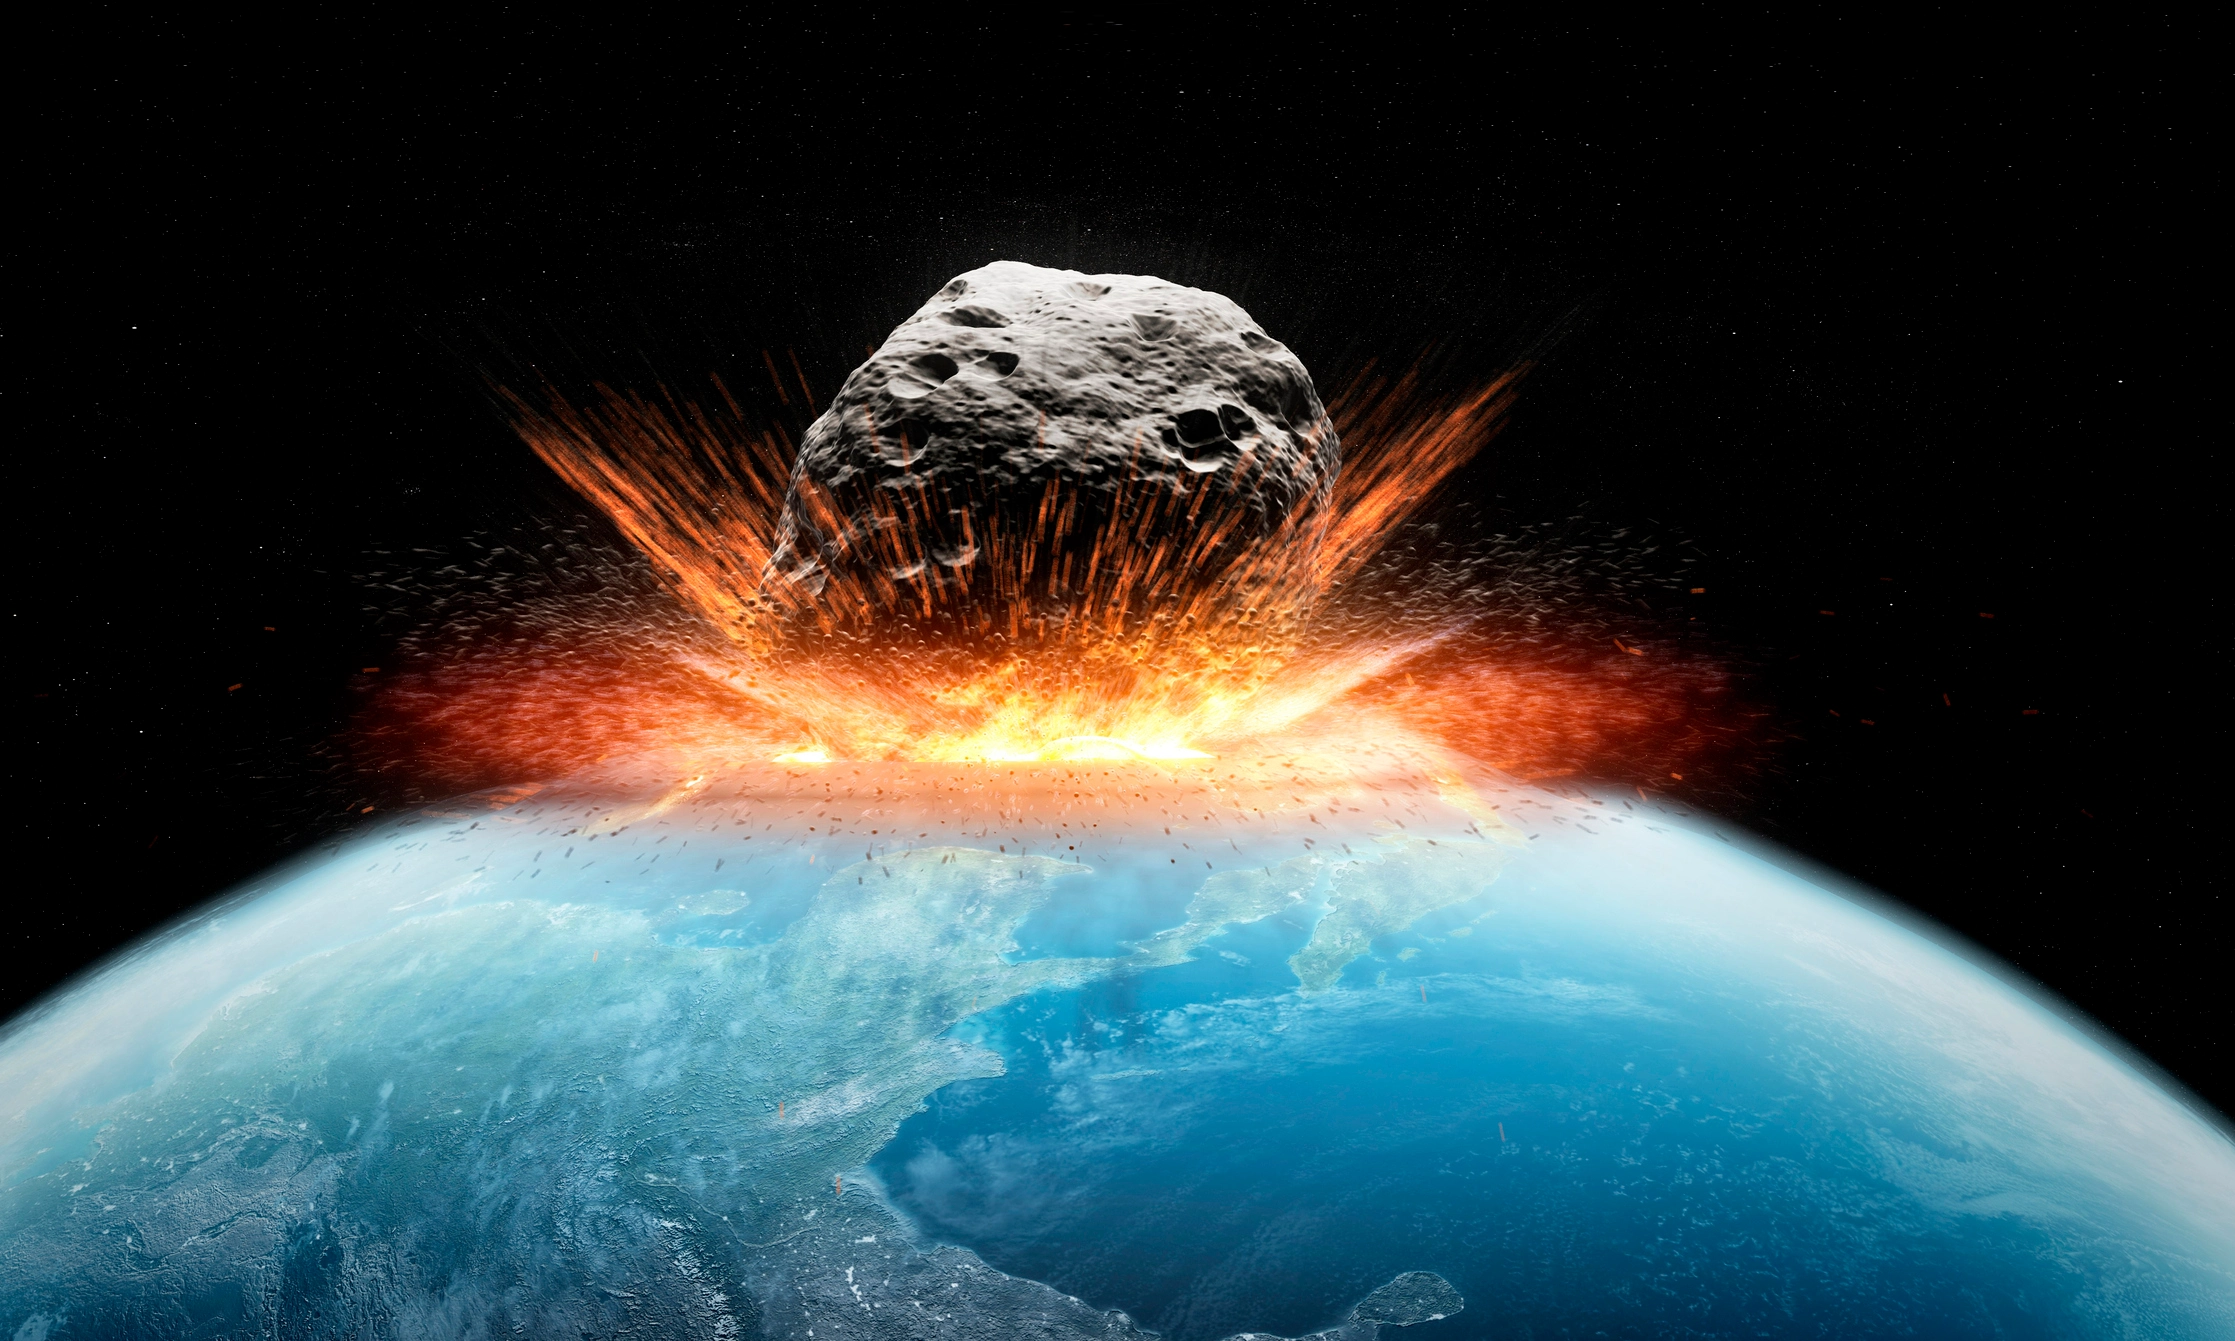
\includegraphics[width=\textwidth]{crash}

    \note{This material is usually stretched over a whole college semester.}
\end{xframe}


\section{Intro}

\begin{xframe}{Objective}
    \begin{itemize}
        \item<1-> Learn core programming concepts
        \item<2-> See practical examples
        \item<3-> Apply concepts in practics
        \item<4-> Provide keywords for google searches
    \end{itemize}

    \note{
        The goal is not to learn how to write any specific code, but rather to learn general concepts.
        These concepts will form a solid foundation for understanding practical code.
        \\
        The practical examples shown are mostly written in GDScript, but the concepts will apply to all languages.
    }
\end{xframe}

\section{Programming Languages}

\begin{xframe}{Languages, Compilers, and Interpreters}
    \begin{itemize}
        \item A programming language is for humans
        \item When written, it's called "code"
        \item Compilers transform code into machine language
        \item Interpreters execute machine code
    \end{itemize}

    \note{Humans write code, a compiler takes that code and converts it into machine language.
    Then, an interpreter, sometimes an actual CPU, executes the machine code.}
\end{xframe}

\begin{xframe}{Scripting Languages}
    \begin{itemize}
        \item Most gamedev is done in scripting languages
        \item Scripts are mainly used to control an existing program
        \item GDScript is Godot's scripting language
    \end{itemize}

    \note{Scripting languages are usually easier to use than other languages.
    They are also great for learning how to code.}
\end{xframe}

\begin{xframe}{Examples of Languages}
    \begin{itemize}
        \item<1-> C/C++ - a "systems language", used in engine code
        \item<2-> JavaScript - used by websites to script the browser
        \item<3-> C\# - server-side code, newfound usage in gamedev
        \item<4-> Lua - generic scripting language used by many games
        \item<5-> Various node-based languages used in gamedev
    \end{itemize}

    \note{There are hundreds of languages.
    Most are all capable of the same tasks, but some are better suited for particular tasks.}
\end{xframe}

\begin{xframe}{Visual Node-based Code}
    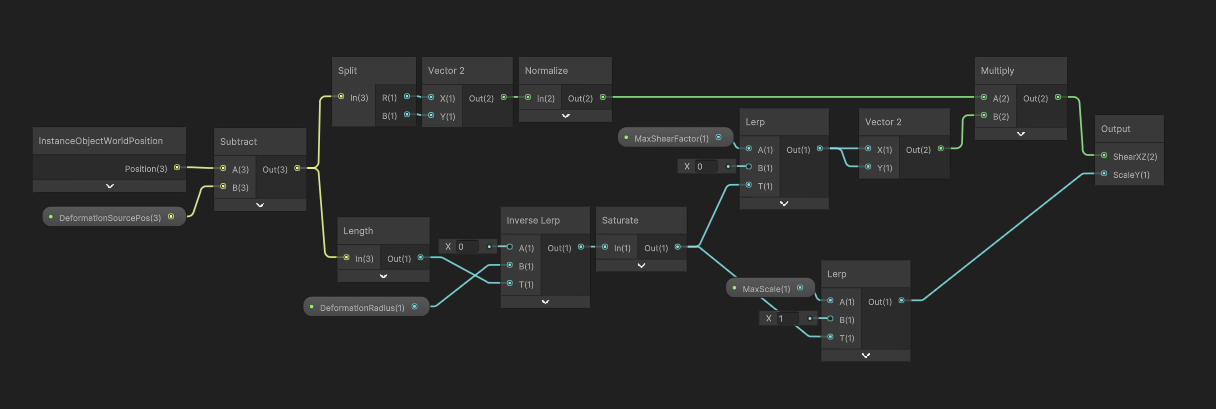
\includegraphics[width=\textwidth]{nodes}

    \note{This is an example of a visual node-based language.
    It is still code, it's just represented in a visual format.
    Artists and designers tend to prefer this kind of language.}
\end{xframe}

\begin{xframe}{Wrapping up Languages}
    \begin{itemize}
        \item When starting a coding project, must pick a language
        \item Most game engines have a scripting language
        \item Most examples will be in GDScript
    \end{itemize}

    \note{Once again, all these core concepts apply to every language.}
\end{xframe}

\section{Language Syntax}

\begin{xframe}{What is Syntax?}
    \begin{itemize}
        \item Syntax is the rules and grammar of the language
        \item Each language has its own syntax
        \item Many languages share certain things
    \end{itemize}

    \note{This is just like human languages, which have punctuation, grammar rules, and sentence structure.}
\end{xframe}

\begin{xframe}{Syntax Examples}

    C++
    \begin{minted}{cpp}
#include <stdio>
int main() {
    std::cout << "Hello, world!" << std::endl;
}
    \end{minted}

    C\#
    \begin{minted}{cs}
using System;

Console.WriteLine("Hello, world!");
    \end{minted}

    GDScript
    \begin{minted}{gd}
print("Hello, world!")
    \end{minted}

    \note{These are all complete programs, which all do the same thing.
    It is not important to understand the code.
    The key takeaway is that the same underlying concepts are present.}
\end{xframe}

\begin{xframe}{What Are Keywords?}
    \begin{itemize}
        \item Words with magic effects
        \item Part of the syntax
        \item Cannot be used for any other purpose
        \item Cannot be used as var names
    \end{itemize}

    \pause
    \bigskip

    Examples from various languages:
    \begin{minted}{text}
func var export and or not for do while if else elif
try finally defer new delete switch case break in of
continue is extends interface implements super const
mut auto local consteval constexpr class struct this
self static extern dynamic public private using enum
protected internal catch continue await yield return
async throw operator enum namespace using
    \end{minted}

    \note{Keywords are built into the grammar of the language.
    They a bit more like punctuation than words.}
\end{xframe}


\begin{xframe}{Some Godot Keywords}
    Highlighted in blue:
    \begin{minted}{gd}
extends Node

export var count: int = 10

func _ready():
    for i in range(count):
        print(i)
        if i == 7:
            break
    \end{minted}

    \note{For the colorblind, the keywords are "extends", "export", "var", "func", "for", "if", and "break".}
\end{xframe}

\begin{xframe}{What Are Comments?}
    \begin{itemize}
        \item Do nothing (non-semantic)
        \item Only for humans
        \item Document the code for teammates and future self
    \end{itemize}

    \pause
    \bigskip

    Example (comments are gray):
    \begin{minted}{gd}
# Called every frame.
func _process(delta):
    pass # Do nothing
    \end{minted}

    \note{The comments are the lines starting with the \#.
    In most languages, the comment is the whole rest of the line.}
\end{xframe}

\section{Values and Types}

\begin{xframe}{What is a Value?}
    \begin{itemize}
        \item Values are pieces of data
        \item Data is represented by bytes
        \item Bytes are like atoms that make up data
        \item Bytes have no inherent meaning, they are just 1s and 0s
    \end{itemize}

    \pause
    \medskip

    Example data, 4 bytes (you don't have to know how to read this):
    \begin{minted}{text}
(binary) 01000111 01000001 01001101 01000101
   (hex)       47       41       4D       45
    \end{minted}

    \pause

    Possible interpretations:

    \begin{columns}
        \begin{column}{0.33\textwidth}
            The integer 1,195,461,957.
        \end{column}
        \begin{column}{0.33\textwidth}
            \onslide<4->{Two items in the player's inventory (each 2 bytes).}
        \end{column}
        \begin{column}{0.33\textwidth}
            \onslide<5->{The text "GAME".}
        \end{column}
    \end{columns}

    \note{The key takeaway here is that the computer doesn't "understand" data.
    Data has no inherent meaning.
    It is humans who give the data meaning.}
\end{xframe}

\begin{xframe}{Sizes of Values}
    \begin{itemize}
        \item Values can be any number of bits
        \item Rounded to next whole number of bytes
        \item A byte is 8 bits
    \end{itemize}

    \pause
    \medskip

    Common numeric data types:
    \medskip

    \begin{tabular}{|c|c|r|} 
        \hline
        Type & Bytes & Value range \\
        \hline
        Boolean & 1 & True or False (1 bit) \\
        \onslide<3->{Byte & 1 & 0 to 255} \\
        Int & 4 & 0 to $\pm 2,147,483,647$ \\
        \onslide<4->{Long Int & 8 & 0 to $\pm 9,223,372,036,854,775,807$} \\
        Float & 4 & 7 digits, 0 to $\pm$\scalebox{0.5}[1]{340,282,370,000,000,000,000,000,000,000,000,000,000} \\
        \onslide<4->{Double & 8 & 16 digits, 0 to $\uparrow$ written 10 times} \\
        \hline
    \end{tabular}

    \note{Memorizing this table is not useful, you can always google it later.
    Just be aware of the general scale of things.}
\end{xframe}

\begin{xframe}{Godot Data Types}
    Just some of Godot's built-in types:
    \medskip

    \begin{tabular}{|c|c|r|} 
        \hline
        Type & Bytes & Value range \\
        \hline
        bool & 1 & true / false \\
        \pause
        int & 8 & 0 to $\pm 9,223,372,036,854,775,807$ \\
        float & 8 & 16 digits, 0 to, like, infinity \\
        \pause
        String & ? & Any Unicode text \\
        \pause
        Vector2 & 2x8 & <X: float, Y: float> \\
        \pause
        Color & 4x8 & <R: float, G: float, B: float, A: float> \\
        \hline
    \end{tabular}

    \note{There are many more types built into Godot, you will pick these up easily.}
\end{xframe}

\begin{xframe}{A Note About Numbers}
    \begin{itemize}
        \item \texttt{int} is limited to integers (-1, 0, 1, 2, 3, ...)
        \item \texttt{float} can store rational numbers (e.g. 42.54634)
        \item A number written with a "point" is a \texttt{float}
        \item A number written without a "point" is a \texttt{int}
    \end{itemize}

    \pause
    \bigskip

    Why not always use \texttt{float} then?
    \begin{itemize}
        \item Cannot store ALL numbers
        \item Sacrifices some precision for range
        \item Cannot reliably store integers past $2^{53}$
        \pause
        \item \texttt{int} can go up to $2^{63}$
        \item \texttt{int} is guaranteed to be an integer
    \end{itemize}

    \note{This is one of the more important things to pay attention to.}
\end{xframe}

\begin{xframe}{Literal Values}
    \begin{itemize}
        \item Literals are written directly into the code
    \end{itemize}

    \begin{minted}{gd}
print(42)
    \end{minted}

    42 is a literal value here.

    \note{Literals are values which don't really exist in memory,
    but instead are stored in the code itself.}
\end{xframe}

\begin{xframe}{Using Values}
    Values can be:
    \begin{itemize}
        \item Overwritten/replaced
        \item Partially modified
        \item Copied
        \item Examined
    \end{itemize}

    \note{Values don't do anything by themselves.
    It's up to the programmer to use them.}
\end{xframe}

\begin{xframe}{Expressions}
    \begin{itemize}
        \item Any piece of code which uses data
        \item Basically any code which *does* something
        \item Defined by the type of the data
        \item The result is stored in temporary data
        \item Some have side effects, such as \texttt{print(x)}
    \end{itemize}

    \pause
    \bigskip

    Examples of expressions:
    \begin{itemize}
        \item a + b
        \item -a
        \item a - (b + c)
        \item \texttt{print(42)}
        \item \texttt{position.x}
        \item \texttt{\$Timer.start(a + b)}
    \end{itemize}

    \note{Expressions are how you use data.
    The available operations available are defined by the data type.
    Expressions result in a piece of temporary data.
    In general, expressions never modify their operands, except for assignment.}
\end{xframe}

\begin{xframe}{Operators}
    \begin{itemize}
        \item Operators are the symbols used to make expressions
        \item Defined by the language
        \item Meaning can change based on data type
    \end{itemize}

    \bigskip

    Examples:
    \begin{itemize}
        \item Math: \texttt{+}, \texttt{-}, \texttt{*}, \texttt{/}
        \item Compare: \texttt{<}, \texttt{>}, \texttt{==}, \texttt{<=}, \texttt{>=}, \texttt{!=}
        \item Function call: \texttt{f(x)}
        \item Member access: \texttt{p.x}
    \end{itemize}
\end{xframe}

\begin{xframe}{Godot's Operators}
    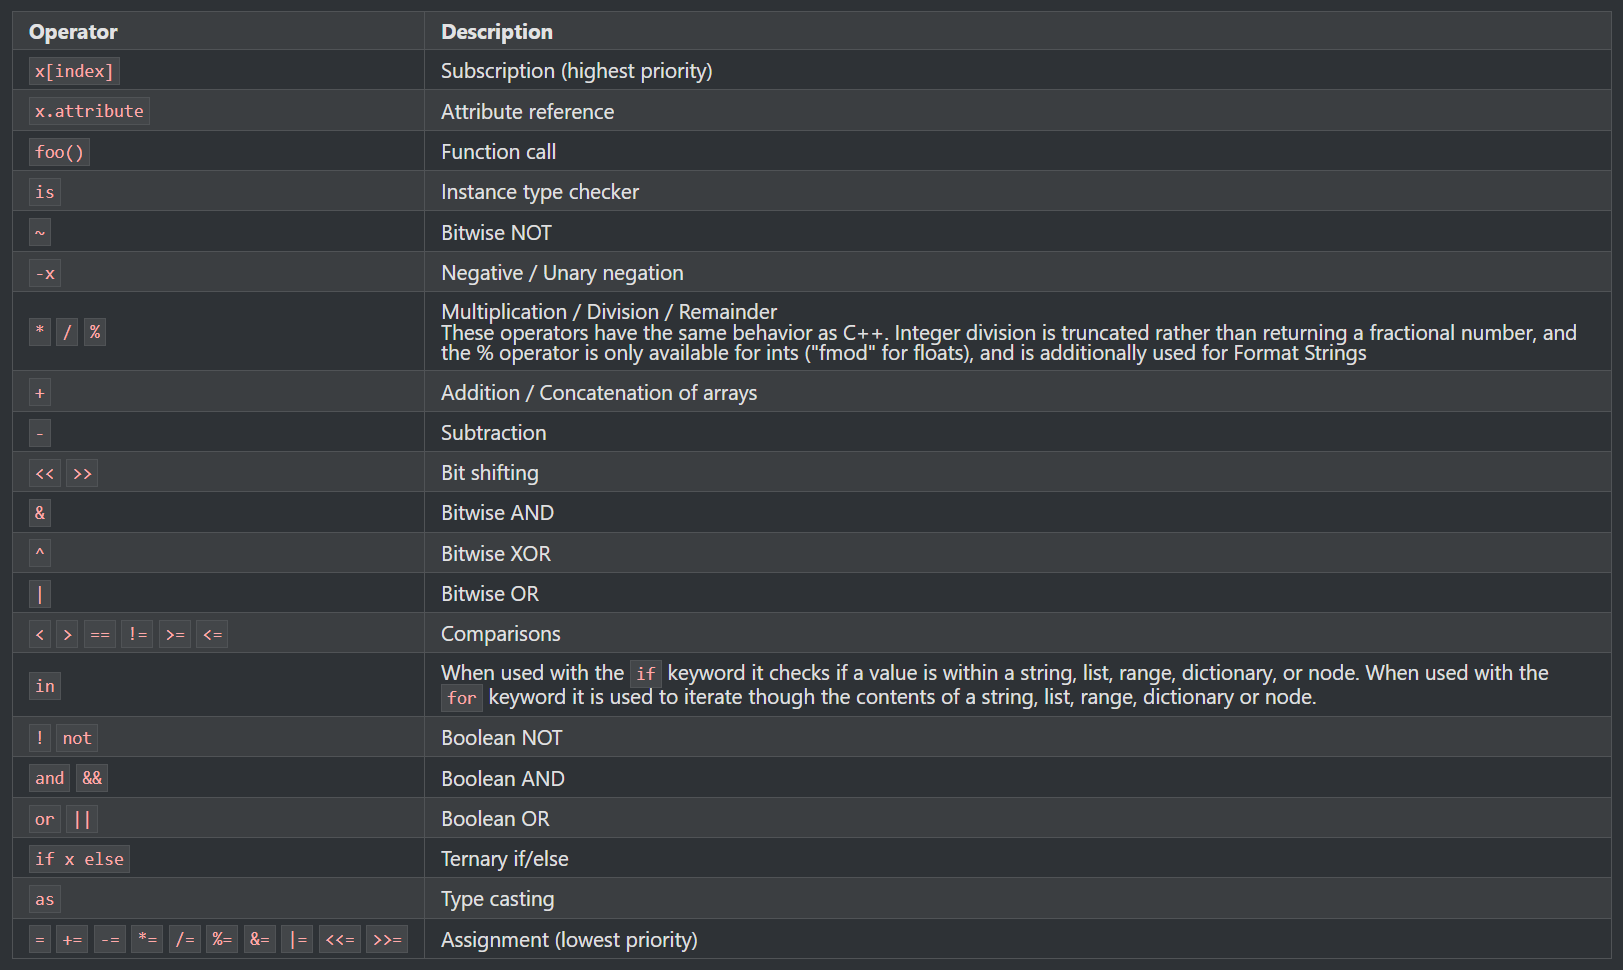
\includegraphics[width=\textwidth]{godot-operators}
\end{xframe}

\begin{xframe}{Types}
    \begin{itemize}
        \item Values always have a specific type
        \item Expressions result in a value of a specific type
    \end{itemize}

    \note{The key thing is that every value and expression is always of a known, specific type.}

    \pause
    \medskip

    A type is defined as:
    \begin{itemize}
        \item The set of possible values
        \item Allowed operations on these values
        \item How the data is represented in memory
    \end{itemize}

    \note{The language has several built-in types which can use more operations,
    but the programmer can create "user-defined" types as well.}

    \pause
    \medskip

    Example of a type:
    \begin{itemize}
        \item Possible values: Integers from -128 to 127
        \item Operations: \texttt{+}, \texttt{-}, \texttt{*}, \texttt{/}
        \item Representation: 8-bit signed binary number in two's complement
    \end{itemize}

    \note{The example type is a signed byte.}
\end{xframe}


\begin{xframe}{Expression Types}
    \begin{itemize}
        \item The result of an expression has a type
        \item The type is determined by the operator and operands
    \end{itemize}

    \pause
    \bigskip

    For example, adding two ints produces an int:
    \begin{minted}{gd}
print(42 + 8) # prints 50
    \end{minted}

    \pause
    \bigskip

    Adding an int and a float produces a float:
    \begin{minted}{gd}
print(42 + 8.0) # prints 50.0
    \end{minted}
\end{xframe}

\begin{xframe}{Type Conversions}
    \begin{itemize}
        \item An operation which converts a value into a different type
        \item Creates a new value of the new type
        \item Never changes the type of the original value
    \end{itemize}

    \pause
    \bigskip

    Example:
    \begin{minted}{gd}
$Label.text = str(42)
# converts (int)42 into (String)"42"
    \end{minted}

    \note{Some languages have more specific syntax for conversions, Godot does not.}
\end{xframe}

\begin{xframe}{Automatic Conversions}
    \begin{itemize}
        \item Happen automatically
        \item Mostly used for numbers
    \end{itemize}

    \pause
    \bigskip

    \begin{minted}{gd}
print(42 * 0.5)
# converts (int)42 into (float)42.0, then multiplies
    \end{minted}

    \note{You should be aware of what automatic conversions are taking place.}
\end{xframe}

\begin{xframe}{Bonfire 1}
    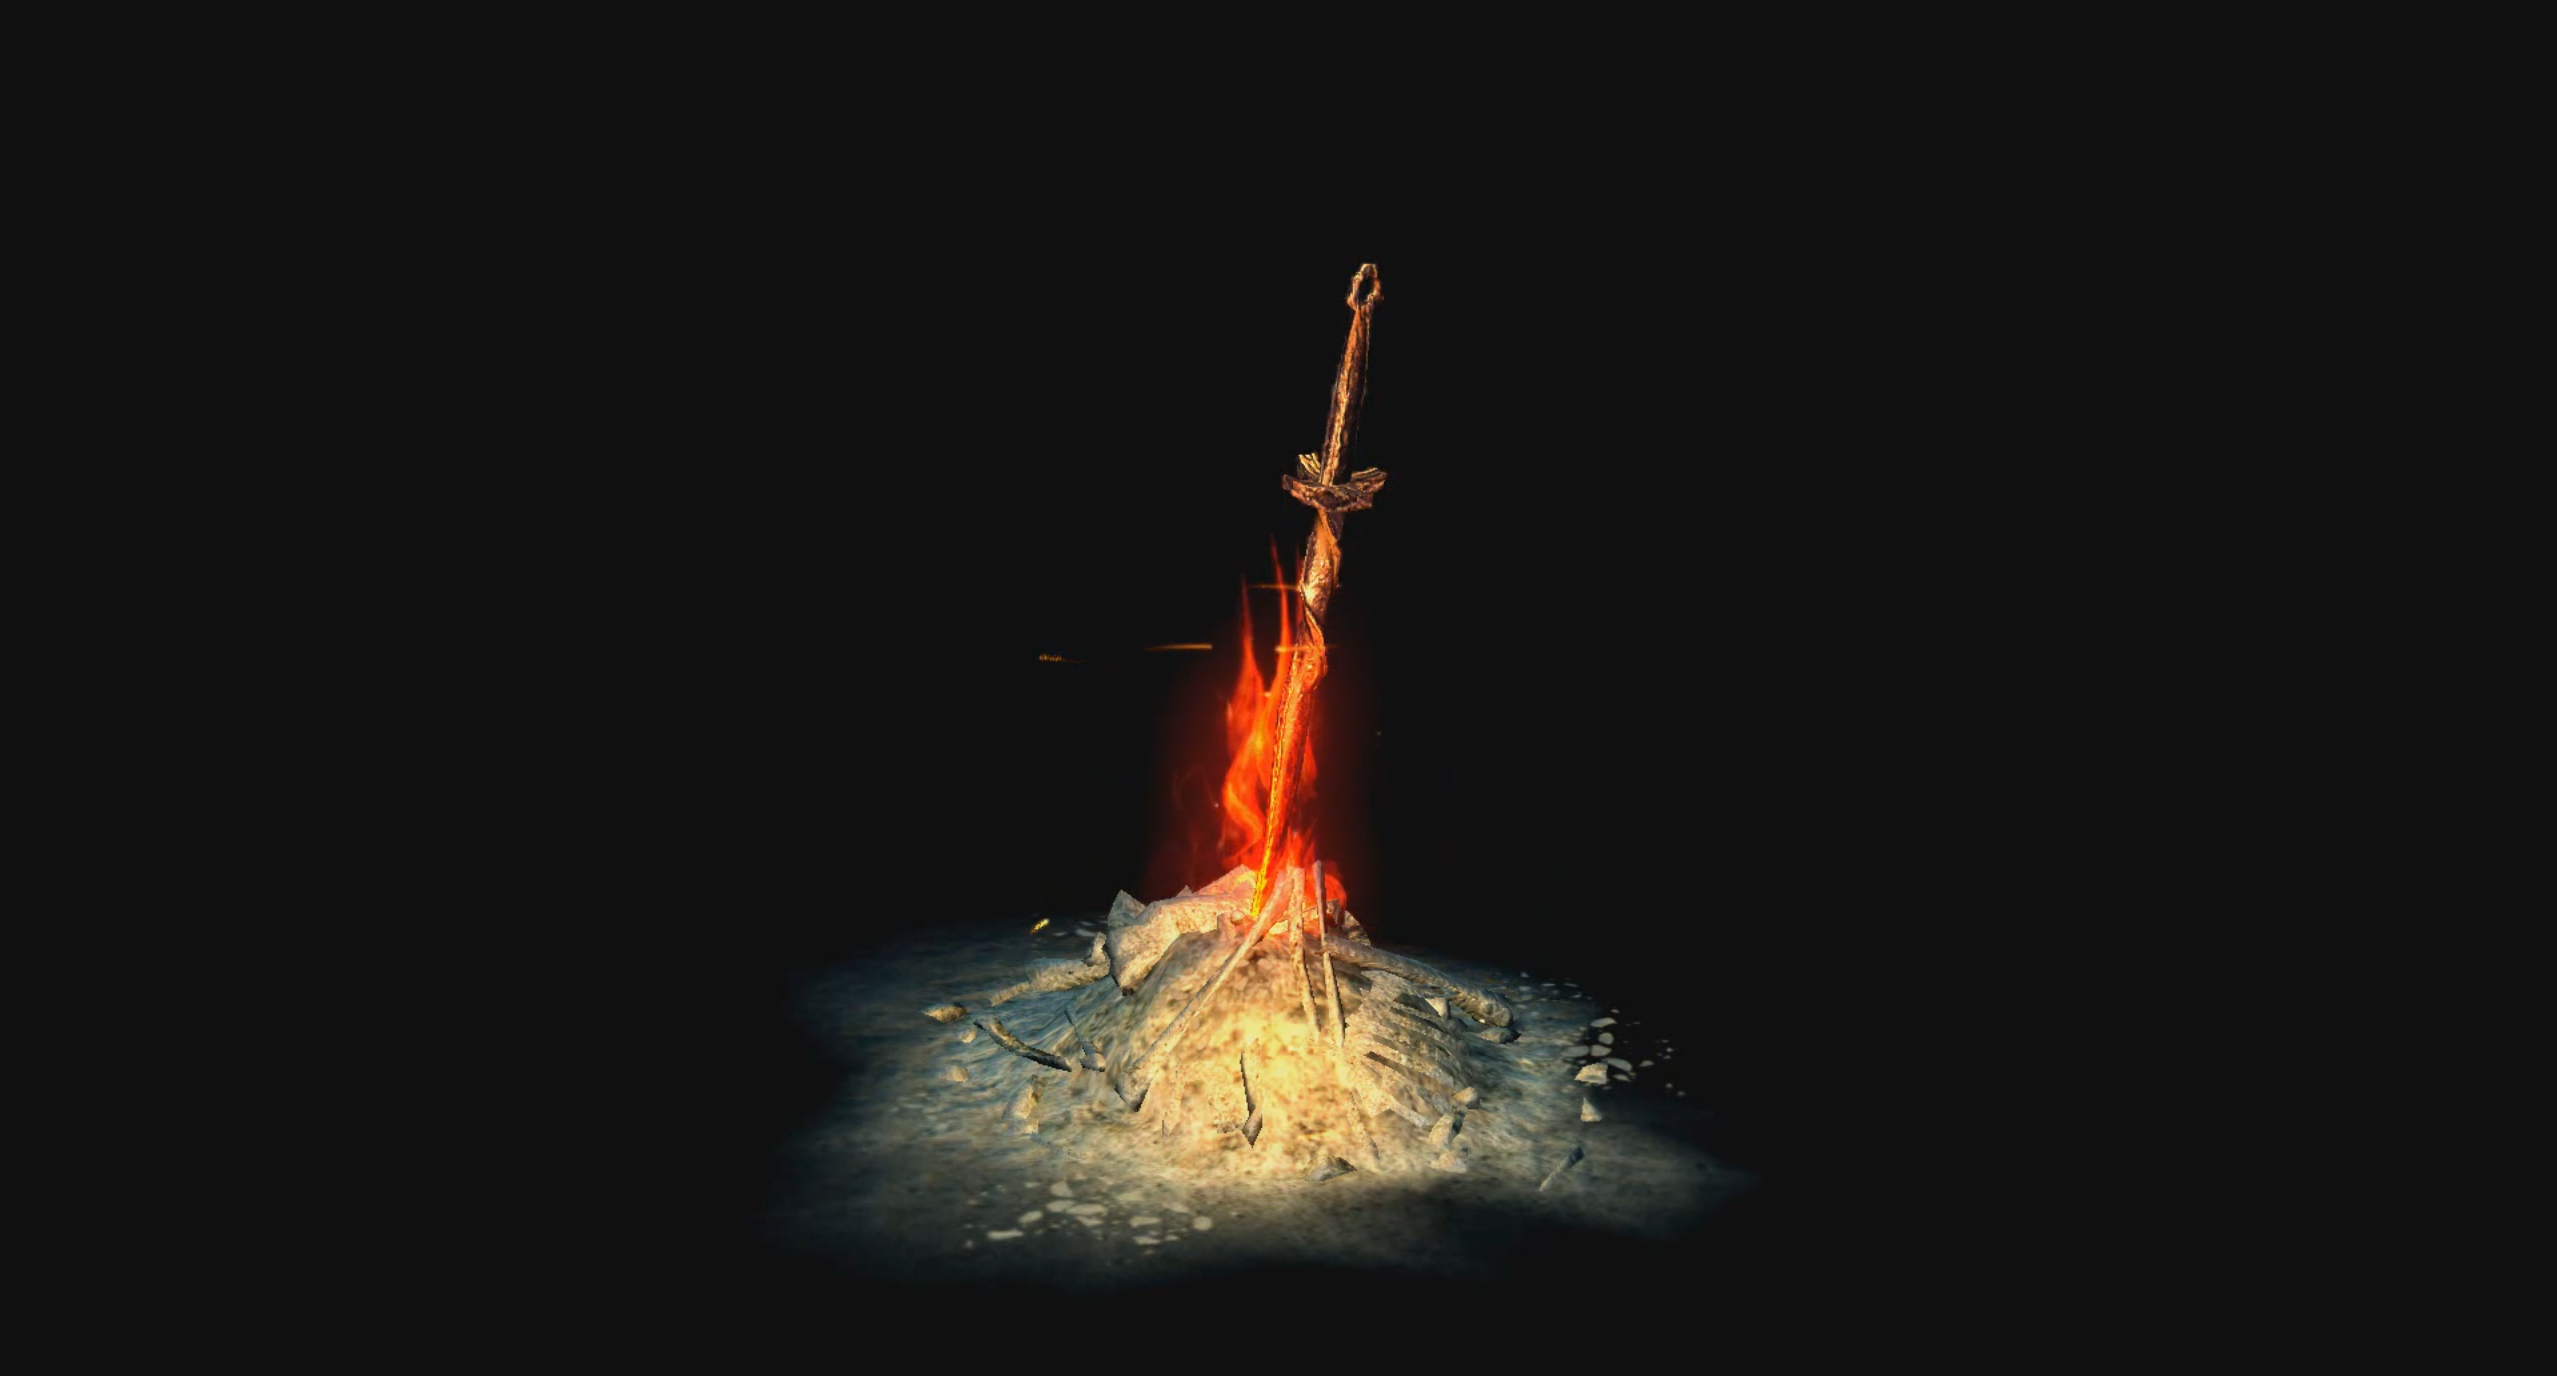
\includegraphics[width=\textwidth]{bonfire}

    \note{Welcome to the bonfire. Use this time to adjust your equipment, spend some souls, and summon som assistance.}
\end{xframe}


\end{document}
